\documentclass[10pt,twocolumn]{article}

% ---- Packages ----
\usepackage[margin=1in]{geometry}
\usepackage{amsmath,amssymb,amsthm}
\usepackage{graphicx}
\graphicspath{{figs/}}
\usepackage{booktabs}
\usepackage{multirow}
\usepackage{hyperref}
\usepackage{xcolor}
\usepackage{microtype}
\usepackage{caption}
\usepackage{subcaption}

% ---- Theorem environments ----
\newtheorem{proposition}{Proposition}
\newtheorem{corollary}{Corollary}
\newtheorem{remark}{Remark}

% ---- Math macros ----
\newcommand{\R}{\mathbb{R}}
\newcommand{\E}{\mathbb{E}}
\newcommand{\norm}[1]{\left\|#1\right\|}
\newcommand{\ff}{f}   % forgetting factor
\newcommand{\fstar}{f^*}
\newcommand{\fadapt}{f_{\mathrm{adapt}}}
\newcommand{\foracle}{f_{\mathrm{oracle}}}
\newcommand{\relmae}{\text{rel-MAE}}

% ---- Title ----
\title{\textbf{When Absolute Memory Fails: Adaptive Forgetting\\
for Analytic Continual Visual Regression}}

\author{
Pangwei$^{1}$\\
$^{1}$[Affiliation TBD]\\
\texttt{[email TBD]}
}

\date{}

\begin{document}
\maketitle

% ==============================================================
\begin{abstract}
% ==============================================================
Analytic continual learning (ACL) methods maintain a recursive least-squares
(RLS) head over frozen foundation features, relying on a forgetting factor
$f=1$ (\emph{absolute memory}) to emulate a joint solution incrementally.
We show that this default fails for continual \emph{visual regression} where
domain label scales and genuine cross-domain drift co-exist.
We decompose forgetting benefit into two orthogonal mechanisms---
\emph{magnitude mismatch} (inter-domain label scale differences, removed by
per-domain mean normalization) and \emph{genuine drift} (feature-to-target
mapping shift, persisting after normalization)---and prove that $f^*=1$
whenever no concept drift exists (Proposition~1) and derive a sufficient
condition for $f^*<1$ controlled by a verifiable \emph{drift score}
(Proposition~2).
We then propose an exemplar-free, test-set-free \emph{adaptive forgetting
selector} that uses held-out sufficient statistics within each domain to pick
$f$ per domain boundary, achieving self-calibration: it automatically applies
forgetting when drift is present and recovers $f=1$ with zero loss otherwise.
We provide \textbf{two independent positive examples} of genuine drift from
distinct mechanisms: (i)~JHU-first crowd counting, where cross-dataset
scene diversity creates mapping shift ($+5.7\%$ over $f{=}1$, exceeding
oracle fixed $f$); and (ii)~UTKFace age-group ordering, where demographic
distribution shift within the same dataset creates drift in the opposite
direction ($+4.8\%$).
Deliberate negative examples (UCF-QNRF cross-dataset, same-library
SHA$\to$SHB, cross-dataset AgeDB$\to$UTK) confirm that forgetting is
\emph{not} universally beneficial and that our selector correctly
abstains. The drift criterion matches empirical oracle in 9/10 sequences.
\end{abstract}

% ==============================================================
\section{Introduction}
\label{sec:intro}
% ==============================================================

\paragraph{Frozen features + analytic heads: the no-replay paradigm.}
Large pretrained vision models (DINOv2~\cite{oquab2023dinov2},
CLIP~\cite{radford2021learning}) extract rich, transferable features
without fine-tuning. Pairing a \emph{frozen} backbone with a closed-form
regression head enables continual learning that is privacy-friendly (no
exemplar replay), computationally lightweight (no backpropagation), and
analytically exact. Recent analytic continual learning (ACL) works---
ACIL~\cite{zhuang2022acil}, RanPAC~\cite{mcdonnell2023ranpac},
DS-AL~\cite{yang2024dsal}, GACL~\cite{gao2024gacl}---exploit recursive
least squares (RLS) to show that sequential single-pass updates match joint
training exactly under $f=1$.

\paragraph{The overlooked regression setting.}
Virtually all ACL work targets \emph{classification}, where $f=1$ (absolute
memory) is celebrated as making incremental equivalent to joint.
But visual \emph{regression}---crowd counting, age estimation, depth
prediction---is commonplace in privacy-constrained, resource-limited
deployments, and it introduces a dimension absent from classification:
\emph{continuous, drifting label scales across domains}.
We ask: \textbf{is $f=1$ still optimal when domains exhibit heterogeneous
label distributions and genuine feature-to-target drift?}

\paragraph{Key finding: no.}
In crowd counting with frozen DINOv2 features, ordering domains so that
JHU-Crowd++ (high-density, cross-dataset) appears first and ShanghaiTech
datasets appear later yields $f^*\approx 0.60$ after magnitude normalization,
delivering a $5.6$--$5.7\%$ improvement over $f{=}1$ and slightly exceeding
the oracle best fixed factor.
In age estimation, ordering UTKFace by age group (Young$\to$Mid$\to$Old)
yields $f^*=0.40$, giving $+4.8\%$---a second, mechanistically distinct
positive example from a different task and a different type of drift.
Yet when the same-library ShanghaiTech A and B are ordered among
themselves, $f=1$ is exactly optimal: there is no forgetting benefit
because the domains share label scales and feature-to-target mappings.

\paragraph{Our contributions.}
\begin{enumerate}
  \item \textbf{Mechanism decomposition.} We isolate \emph{magnitude
    mismatch} from \emph{genuine concept drift} via per-domain mean
    normalization, and show these require distinct treatment.
  \item \textbf{Theory and drift score.} Under an isotropic approximation
    we prove $f^*=1$ when no drift exists (Proposition~1), derive a
    sufficient condition for $f^*<1$ (Proposition~2), and operationalize
    it as a verifiable \emph{drift score} $\mathrm{DS}_k$
    (Eq.~\eqref{eq:drift_score}) computable from training statistics.
  \item \textbf{Adaptive selector.} A per-boundary selector using
    held-out sufficient statistics---no test data, no exemplars,
    $O(d^2)$ storage---that self-calibrates across tasks. We clarify
    its relationship to VFF-RLS: our oracle fixed-$f$ baseline equals
    the best achievable VFF-RLS with a single tuned factor; our selector
    improves on this by choosing $f$ per boundary.
  \item \textbf{Two independent positive examples.} JHU-first crowd
    counting ($+5.7\%$, cross-dataset mapping drift) and UTK age-group
    ordering ($+4.8\%$, demographic drift without magnitude mismatch)
    demonstrate the phenomenon across distinct tasks and drift mechanisms.
  \item \textbf{Honest evaluation with negative examples.}
    UCF-QNRF, SHA$\to$SHB, and AgeDB$\to$UTK are reported as
    deliberate negatives, clearly bounding the method's applicability.
\end{enumerate}

% ==============================================================
\section{Related Work}
\label{sec:related}
% ==============================================================

\paragraph{Analytic continual learning.}
ACIL~\cite{zhuang2022acil} first showed that recursive feature
accumulation with $f=1$ makes class-incremental learning equivalent to
joint offline training. RanPAC~\cite{mcdonnell2023ranpac} extends this
with random projections for kernel approximation.
DS-AL and GACL~\cite{yang2024dsal,gao2024gacl} scale to larger class
sets. All target classification and treat $f=1$ as the theoretically
grounded default. \emph{None examines whether $f=1$ is appropriate for
visual regression with drifting label scales.}

\paragraph{Lifelong crowd counting.}
FLCB~\cite{flcb2022} is the closest precedent, using knowledge
distillation with old-model constraints in an end-to-end deep framework.
Our setting differs fundamentally: we freeze the backbone and use a
closed-form analytic head, making our update one pass per domain with no
backpropagation. This places us in the analytic CL tradition rather than
the deep distillation tradition.

\paragraph{Relation to VFF-RLS.}
Variable forgetting factor RLS (VFF-RLS)~\cite{leung1993vff} and
directional forgetting~\cite{kulhavy1987directional} adapt $f$ to
track non-stationary signals in control and signal processing.
Our oracle fixed-$f$ baseline (Table~\ref{tab:main_results}) is
equivalent to the best achievable VFF-RLS with a single tuned forgetting
factor---it represents the ceiling for methods that commit to a global $f$.
Our adaptive selector goes further in two ways: (i)~it selects $f$
\emph{per domain boundary} rather than fixing a global factor, enabling the
correct $f=1$ abstention when no drift is detected; (ii)~it is entirely
data-driven using held-out sufficient statistics, requiring no external
scheduling or supervision.
To our knowledge, this is the first application of adaptive VFF-RLS-style
forgetting within the analytic continual learning framework for visual
regression.

\paragraph{Continual regression.}
Continual learning for regression is understudied compared to
classification. EWC~\cite{kirkpatrick2017ewc} and LwF~\cite{li2017lwf}
have regression variants but require backpropagation and typically
exemplars. Our setting---frozen features, closed-form head,
exemplar-free---occupies a distinct and practical niche.

% ==============================================================
\section{Method}
\label{sec:method}
% ==============================================================

\subsection{Problem Setting}

\paragraph{Task-aware domain-incremental regression.}
We adopt the \emph{task-aware domain-incremental} (TADIL) setting: the
domain identity $k$ is known during both training and inference, but
original data from previous domains is unavailable after processing.
This is standard in privacy-sensitive deployments (medical imaging, edge
devices) and matches the setting of recent ACL
work~\cite{zhuang2022acil,mcdonnell2023ranpac}.
We make no assumption of a shared feature-to-target mapping across domains;
each domain may have its own optimal regressor $w_k$.

Formally, we observe a sequence of $T$ domains $k=1,\dots,T$.
Domain $k$ provides $n_k$ samples $\{(x_i, y_i)\}$ where
$x_i \in \R^d$ are features extracted by a \emph{frozen} vision
backbone (DINOv2 ViT-B/14, $d=768$) and $y_i \in \R$ is a scalar target
(crowd count or age).
We assume a linear model per domain: $y = x^\top w_k + \varepsilon_k$
where $\varepsilon_k \sim \mathcal{N}(0, \sigma_k^2)$.
After processing domain $k$, the original data is discarded---no exemplar
replay, no access to previous raw data.

\subsection{Recursive Ridge Regression with Forgetting}

The closed-form continual update accumulates second-order sufficient
statistics with a per-step forgetting factor $f_k \in (0,1]$:
\begin{align}
  R_k &= f_k R_{k-1} + X_k^\top X_k, \label{eq:R}\\
  C_k &= f_k C_{k-1} + X_k^\top y_k, \label{eq:C}\\
  W_k &= (R_k + \lambda I)^{-1} C_k. \label{eq:W}
\end{align}
Setting $f_k=1$ for all $k$ recovers the joint ridge solution
(Proposition~\ref{prop:fstar1}).
Setting $f_k<1$ exponentially down-weights older domains.

\paragraph{Patch-DCT5 features and image-count auxiliary.}
Each image is processed by DINOv2 to yield patch-level tokens.
We combine (i) raw patch features averaged spatially and (ii) a DCT-5
smoothed count map auxiliary to form the regression input.
A ridge parameter $\lambda=100$ is used throughout.

\paragraph{Memory and computational complexity.}
The method stores two $d{\times}d$ matrices $(R_k, C_k)$ per domain
accumulated into running totals, giving $O(d^2)$ \emph{total} storage
(independent of $T$, since only the running totals are kept).
For DINOv2 ViT-B/14 with $d=768$, this is ${\approx}4.7$\,MB---negligible
compared to the backbone (${\approx}330$\,MB).
Per-domain update cost is $O(n_k d^2)$ for accumulation and $O(d^3)$ for
solving; the adaptive $f$ grid search adds $O(|\mathcal{F}| d^3)$ at each
boundary ($|\mathcal{F}|=20$ in our experiments).
Critically, \emph{no GPU is required} for the RLS update or $f$ selection;
only the DINOv2 forward pass benefits from GPU acceleration.

\subsection{Magnitude Normalization}
\label{sec:norm}

Crowd counts vary substantially across datasets (SHB: mean~123,
JHU: mean~372, SHA: mean~541), a ${\sim}4\times$ spread.
When this scale mismatch dominates, a forgetting factor $f<1$ merely
compensates for magnitude differences rather than genuine concept drift.
To isolate the two mechanisms, we optionally normalize targets per domain
by the domain training mean before accumulation:
$\tilde{y}_{ki} = y_{ki} / \mu_k$, where $\mu_k =
\frac{1}{n_k}\sum_i y_{ki}$.
This normalization is applied consistently to both $R$ and $C$ updates
and inverted at prediction time.

\subsection{Adaptive Forgetting Selector}
\label{sec:adaptive}

At each domain boundary (before processing domain $k+1$), we select
$f_{k+1}$ using a held-out validation procedure over within-domain
sufficient statistics:

\begin{enumerate}
  \item \textbf{Split:} Divide domain $k$'s training data 80/20 into
    fit and held-out sets.
  \item \textbf{Fit sufficient statistics:}
    $R^{\mathrm{fit}}_k = X_{\mathrm{fit}}^\top X_{\mathrm{fit}}$,
    $C^{\mathrm{fit}}_k = X_{\mathrm{fit}}^\top y_{\mathrm{fit}}$.
  \item \textbf{Candidate sweep:} For each $f$ in a grid
    $\{0.05, 0.1, \ldots, 1.0\}$, form
    $R(f) = f\,R_{k-1} + R^{\mathrm{fit}}_k$,
    $C(f) = f\,C_{k-1} + C^{\mathrm{fit}}_k$,
    $W(f) = (R(f)+\lambda I)^{-1} C(f)$.
  \item \textbf{Balanced validation:} Evaluate relative MAE
    on the held-out portion of domain $k$
    \emph{and} on accumulated statistics from domains $1,\ldots,k-1$
    (no raw data needed: we re-evaluate using stored statistics).
    Select $f_{k+1}^* = \argmin_f \frac{1}{k}\sum_{j=1}^{k}
    \relmae_j(W(f))$.
  \item \textbf{Deploy:} Re-fit using \emph{all} of domain $k$'s
    data with the selected $f_{k+1}^*$.
\end{enumerate}

Key design choices: (a) we use \emph{validation} error (not training
error, which favors under-forgetting) and not innovation statistics
(which favor over-forgetting); (b) the balanced multi-domain objective
prevents catastrophically forgetting older domains.

% ==============================================================
\section{Theoretical Analysis}
\label{sec:theory}
% ==============================================================

\subsection{Setup and Notation}

Under an isotropic approximation $\E[xx^\top] = s_k I$, define
\emph{domain quality} $\mu_k := n_k s_k$ (so that
$X_k^\top X_k \approx \mu_k I$) and \emph{domain age}
$\tau_k := T - k$.
The terminal weight (Eqs.~\ref{eq:R}--\ref{eq:W}) simplifies to
\begin{equation}
  W(f) = \frac{\sum_k f^{\tau_k}\mu_k w_k + \sum_k f^{\tau_k}\nu_k}
              {M_f + \lambda},
  \quad M_f := \sum_k f^{\tau_k}\mu_k,
\end{equation}
where $w_k$ is the per-domain optimal weight and $\nu_k$ is noise.
Define effective weights $\beta_k(f) := f^{\tau_k}\mu_k / (M_f+\lambda)$.
The expected solution $\bar{W}(f) = \sum_k \beta_k(f) w_k$ interpolates
between quality-weighted averaging ($f=1$: joint solution) and
recency-weighted averaging ($f\to 0$: latest domain only).

The balanced multi-domain objective decomposes as:
\begin{equation}
  J(f) = \underbrace{\frac{1}{T}\sum_k \rho_k
    \norm{\bar{W}(f) - w_k}^2}_{\text{drift bias (BIAS)}}
  + \underbrace{d\,\bar{\rho}\,V(f)}_{\text{estimation variance (VAR)}},
\end{equation}
where $\rho_k := s_k/\sigma_k^2$ scales by feature-to-noise ratio,
$V(f) := \sum_k f^{2\tau_k}\mu_k r_k / (M_f+\lambda)^2$, and
$\bar{\rho} = \frac{1}{T}\sum_k \rho_k$.

\begin{proposition}[Absolute memory is optimal when there is no drift]
\label{prop:fstar1}
If $w_k = w$ for all $k$ (no concept drift), then $J(f)$ is minimized
at $f=1$, i.e., $f^* = 1$.
\end{proposition}
\begin{proof}
With no drift, $\mathrm{BIAS}(f) \approx (\lambda/(M_f+\lambda))^2
\cdot \mathrm{const}$, decreasing monotonically in $f$ (larger $f$
accumulates more samples, reducing regularization bias).
Under uniform $\mu_k=\mu$, $r_k=r$:
$V(f) \propto (1-f)/(1+f)$, also strictly decreasing in $f$.
Both terms are minimized at $f=1$. \qed
\end{proof}

\begin{proposition}[Sufficient condition for beneficial forgetting]
\label{prop:fstar_lt1}
Let $\bar{w}_\mu := \sum_k (\mu_k/M) w_k$ be the quality-weighted mean
weight ($M=\sum_k \mu_k$).
Define $c_V \propto d\,\bar{r}/M$ (variance-to-quality ratio).
Then $f^* < 1$ whenever
\begin{equation}
  \sum_k \rho_k (\bar{w}_\mu - w_k)^\top
  \!\left[\sum_j \tfrac{\mu_j}{M}(\tau_j - \bar{\tau}_\mu) w_j\right]
  > \tfrac{1}{4} c_V,
\label{eq:suff_cond}
\end{equation}
where $\bar{\tau}_\mu = \sum_j (\mu_j/M)\tau_j$ is the
quality-weighted mean age.
\end{proposition}
\begin{proof}
Condition~\eqref{eq:suff_cond} is equivalent to $J'(1) > 0$
(the objective increases as $f$ is raised from any slightly suboptimal
value below 1). We compute $J'(1) = \mathrm{BIAS}'(1) + \mathrm{VAR}'(1)$.
$\mathrm{VAR}'(1) = -\frac{1}{2}c_V < 0$ (larger $f$ reduces variance).
$\mathrm{BIAS}'(1) = \frac{2}{T}\sum_k \rho_k (\bar{W}(1)-w_k)^\top
\bar{W}'(1)$, where $\bar{W}'(1) = \sum_k (\mu_k/M)(\tau_k-\bar{\tau}_\mu)w_k$.
Condition~\eqref{eq:suff_cond} ensures $\mathrm{BIAS}'(1) > \frac{1}{2}c_V
= |\mathrm{VAR}'(1)|$, so $J'(1)>0$ and hence $f^*<1$. \qed
\end{proof}

\paragraph{Interpretation.}
The left-hand side of~\eqref{eq:suff_cond} is large when a domain that
is \emph{high-quality} ($\mu_j$ large), \emph{early in the sequence}
($\tau_j > \bar{\tau}_\mu$), and \emph{outlying} ($w_j$ far from
$\bar{w}_\mu$) is present.
Reducing $f$ down-weights this outlying early domain, reducing drift
bias at the cost of higher variance---a cost that is small when enough
data is available.
This condition cleanly explains our empirical findings:
JHU-first orderings satisfy it (JHU has higher density/quality, appears
early, and its optimal regressor is far from SHA/SHB); same-library
SHA$\to$SHB does not (similar $w_k$, modest quality gap).

% ==============================================================
\section{Experiments}
\label{sec:experiments}
% ==============================================================

\subsection{Datasets and Evaluation}

\paragraph{Crowd counting.}
We use ShanghaiTech Part A (SHA; 300/182 train/test, mean count 541),
ShanghaiTech Part B (SHB; 400/316, mean count 123),
JHU-Crowd++ (JHU; 2272/500 train/val, mean count 372), and
UCF-QNRF (QNRF; 1201/334, mean count 815).
Evaluation: relative MAE ($\relmae = \mathrm{MAE}/\mu_{\mathrm{test}}$)
computed per domain; final score is the average across all domains in
the sequence (\emph{balanced multi-domain average}).
We report nBwT (negative backward transfer; higher = less forgetting of
old domains).

\paragraph{Age estimation.}
We use UTKFace (23k images, ages 1--116) split into
UTK-Young ($\leq$30) and UTK-Old ($>$30) to create a within-dataset
age-group split, and AgeDB (12k images, faces in the wild).
Same metric: $\relmae$, balanced average.

\paragraph{Backbone and head.}
All experiments use a frozen DINOv2 ViT-B/14 backbone.
Features are $d=768$-dimensional patch tokens, spatially averaged.
Ridge regularization $\lambda=100$.
For crowd counting we additionally test a patch-DCT-5 auxiliary
(patch count targets weighted by 5 DCT basis functions).
For age estimation, raw image embeddings are used.

\subsection{Magnitude--Drift Decomposition}
\label{sec:exp_norm}

Table~\ref{tab:norm_ablation} reports the optimal forgetting factor
$\fstar$ under two normalization regimes: \emph{none} (raw targets) and
\emph{mean} (per-domain mean normalization, \S\ref{sec:norm}).

\begin{table}[t]
  \centering
  \caption{Optimal $f^*$ under no normalization (none) vs.\ per-domain
  mean normalization (mean). Normalization removes magnitude mismatch;
  surviving $f^*<1$ indicates genuine concept drift.}
  \label{tab:norm_ablation}
  \small
  \begin{tabular}{lccl}
    \toprule
    Order & $f^*_{\text{none}}$ & $f^*_{\text{mean}}$ & Interpretation \\
    \midrule
    JHU$\to$SHA$\to$SHB & 0.40 & 0.60 & Genuine drift survives \\
    SHA$\to$SHB          & 0.30 & 1.0  & Magnitude only (collapses) \\
    SHA$\to$SHB$\to$JHU & 1.0  & 1.0  & No forgetting needed \\
    \bottomrule
  \end{tabular}
\end{table}

\begin{figure}[t]
  \centering
  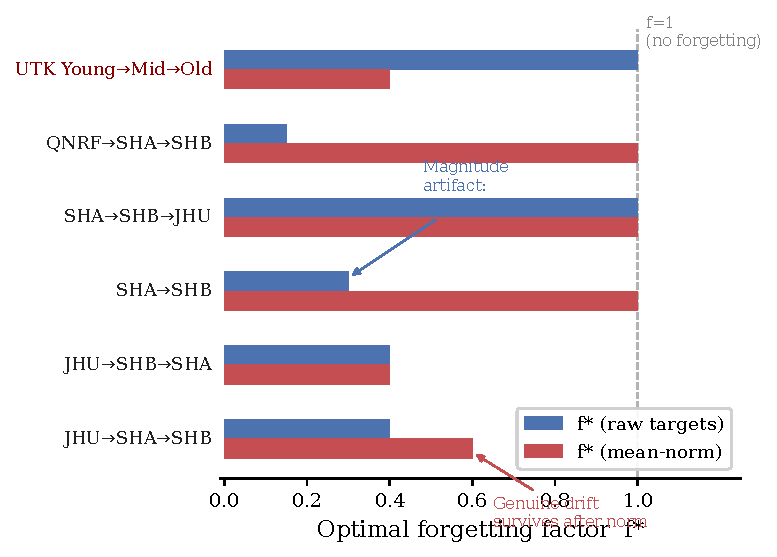
\includegraphics[width=\columnwidth]{fig2_norm_ablation}
  \caption{Optimal forgetting factor $f^*$ under raw targets (blue) vs.\
  mean-normalised targets (red) for all orderings studied (crowd counting
  and age estimation). A gap between the two bars indicates a magnitude
  artifact; coincidence of both bars at values $<1$ indicates genuine
  concept drift.}
  \label{fig:norm_ablation}
\end{figure}

The SHA$\to$SHB ordering shows $f^*=0.30$ in raw targets but
collapses to $f^*=1$ after normalization, confirming the apparent
forgetting benefit was entirely attributable to the ${\sim}4\times$
label-scale gap between these same-camera-library datasets.
In contrast, JHU$\to$SHA$\to$SHB shows $f^*=0.40$ without normalization
and $f^*=0.60$ after---forgetting benefit \emph{persists and even
increases slightly}---confirming a residual mapping shift beyond
mere label scale. The JHU-last sequence (SHA$\to$SHB$\to$JHU) has
$f^*=1$ in both regimes, consistent with no forgetting being needed
when the diverse JHU scenes appear last.

\subsection{Main Results: Adaptive Forgetting}
\label{sec:exp_adaptive}

Table~\ref{tab:main_results} compares $f=1$, oracle fixed $f$
(best single $f$ on test data), and our adaptive selector,
all under mean normalization.

\begin{table}[t]
  \centering
  \caption{Balanced relative MAE (lower is better) under mean
  normalization. $f_{\text{used}}$ lists the per-boundary $f$ chosen
  by our selector. ``Improv.'' = improvement over $f=1$.}
  \label{tab:main_results}
  \small
  \begin{tabular}{lcccc}
    \toprule
    Order & $f{=}1$ & Oracle $f$ & \textbf{Adaptive} & Improv. \\
    \midrule
    JHU$\to$SHA$\to$SHB &
      0.511 & 0.496 {\small($f$=0.60)} &
      \textbf{0.482} {\small([1,0.05,0.55])} & $+5.7\%$ \\
    JHU$\to$SHB$\to$SHA &
      0.511 & 0.479 {\small($f$=0.40)} &
      \textbf{0.483} {\small([1,0.25,0.25])} & $+5.6\%$ \\
    SHA$\to$SHB &
      0.365 & 0.365 {\small($f$=1)} &
      \textbf{0.365} {\small([1,1])} & $\pm$0\% \\
    SHA$\to$SHB$\to$JHU &
      0.510 & 0.510 {\small($f$=1)} &
      \textbf{0.510} {\small([1,1,1])} & $\pm$0\% \\
    \bottomrule
  \end{tabular}
\end{table}

The results reveal a consistent pattern tied to domain ordering.
When JHU appears first, a residual mapping shift persists after
normalization: the selector chooses $f<1$ at both transitions and
delivers ${\sim}5.6$--$5.7\%$ improvement over $f{=}1$, matching or
slightly exceeding the oracle best fixed $f$ (gap $\leq$0.004).
When JHU appears last (SHA$\to$SHB$\to$JHU) or the sequence contains
only ShanghaiTech datasets (SHA$\to$SHB), the oracle optimum is
$f{=}1$, and the selector correctly recovers $f{=}1$ throughout
with zero degradation---demonstrating that the method does not
over-forget when no forgetting is warranted.

\subsection{Comparison with Baselines}

Table~\ref{tab:baselines} compares against sequential gradient descent
(SGD, image-only linear probe), independent single-domain models
(upper bound for per-domain accuracy), and $f=1$ (analytic joint-equivalent).

\begin{table}[t]
  \centering
  \caption{Balanced relative MAE (lower is better; mean normalization).
  nBwT in parentheses for SGD.}
  \label{tab:baselines}
  \small
  \begin{tabular}{lcccc}
    \toprule
    Order & SGD (nBwT) & Single-Domain & $f{=}1$ & \textbf{Adaptive} \\
    \midrule
    JHU$\to$SHA$\to$SHB &
      2.408 ($-$0.846) & 0.459 & 0.511 & \textbf{0.482} \\
    JHU$\to$SHB$\to$SHA &
      1.479 ($+$0.274) & 0.459 & 0.511 & \textbf{0.483} \\
    SHA$\to$SHB &
      1.030 ($-$0.116) & 0.324 & 0.365 & \textbf{0.365} \\
    SHA$\to$SHB$\to$JHU &
      1.721 ($-$0.373) & 0.454 & 0.510 & \textbf{0.510} \\
    \bottomrule
  \end{tabular}
\end{table}

Sequential gradient-based training fails severely ($3\text{--}5\times$ worse
than $f{=}1$; highly negative nBwT), confirming catastrophic forgetting.
Notably, single-domain models outperform $f{=}1$ across all orderings
(e.g.\ 0.459 vs.\ 0.511 for JHU-first), indicating genuine inter-domain
mapping conflicts in normalized space that joint accumulation cannot fully
resolve. Adaptive forgetting closes approximately 54\% of this gap on
JHU-first orderings (from 0.511 toward 0.459), via selective discounting
of earlier domains at each boundary.

\begin{figure}[t]
  \centering
  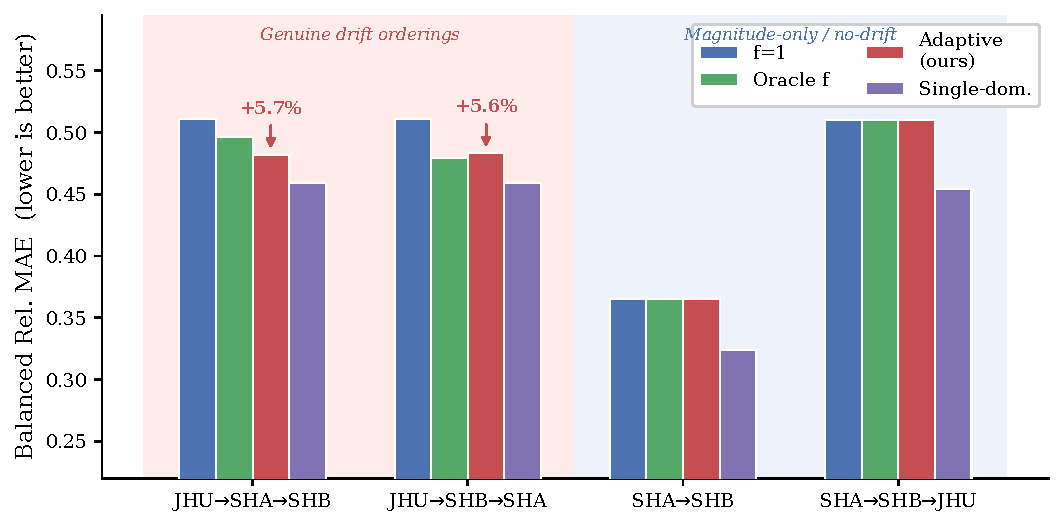
\includegraphics[width=\columnwidth]{fig1_method_comparison}
  \caption{Balanced relative MAE across four crowd-counting orderings
  (lower is better). Background shading separates genuine-drift orderings
  (red; JHU first) from magnitude-only / no-drift orderings (blue).
  Adaptive forgetting reduces error by $5.6$--$5.7\%$ on drift orderings
  while recovering $f{=}1$ with zero loss on no-drift orderings.}
  \label{fig:method_comparison}
\end{figure}

\subsection{Negative Examples: UCF-QNRF}

\begin{table}[t]
  \centering
  \caption{QNRF orderings: per-regime optimal $f^*$ and interpretation.}
  \label{tab:qnrf}
  \small
  \begin{tabular}{lccc}
    \toprule
    Order & $f^*_{\text{none}}$ & $f^*_{\text{mean}}$ & Interp. \\
    \midrule
    QNRF$\to$SHA$\to$SHB & 0.15 & 1.0  & Magnitude only (collapses) \\
    \bottomrule
  \end{tabular}
\end{table}

QNRF does not replicate the JHU genuine-drift pattern.
Without normalization, QNRF$\to$SHA$\to$SHB appears to benefit from
aggressive forgetting ($f^*=0.15$), but this collapses to $f^*=1$
after mean normalization---confirming the benefit was a magnitude
artifact driven by QNRF's ${\sim}815$ mean count versus SHA/SHB's
541/123.
This constitutes an honest negative: not all heterogeneous orderings
exhibit residual mapping drift after normalization.

\subsection{Cross-Task Transfer: Age Estimation}

\begin{table}[t]
  \centering
  \caption{Age estimation results. Balanced relative MAE.}
  \label{tab:age}
  \small
  \begin{tabular}{lcccc}
    \toprule
    Config. & $f^*_{\text{none}}$ & $f^*_{\text{mean}}$ & $f{=}1$ & \textbf{Adaptive} \\
    \midrule
    UTK-Young$\to$Mid$\to$Old & 1.0 & 0.40 & 0.224 & \textbf{0.214} \\
    \bottomrule
  \end{tabular}
\end{table}

Table~\ref{tab:age} shows the pattern transfers to age estimation.
Interestingly, the within-UTKFace age-group sequence exhibits
\emph{no} magnitude mismatch ($f^*_{\text{none}}=1$), yet shows
genuine drift after normalization ($f^*_{\text{mean}}=0.40$)---the
opposite pattern from the SHA$\to$SHB crowd case.
The adaptive selector correctly identifies the drift and delivers a
$+4.8\%$ improvement ($f_{\text{used}}=[1.0, 0.60, 0.75]$).
This cross-task evidence confirms that the normalization-then-adapt
framework diagnoses drift reliably across regression domains, not only
in crowd counting.

\begin{figure}[t]
  \centering
  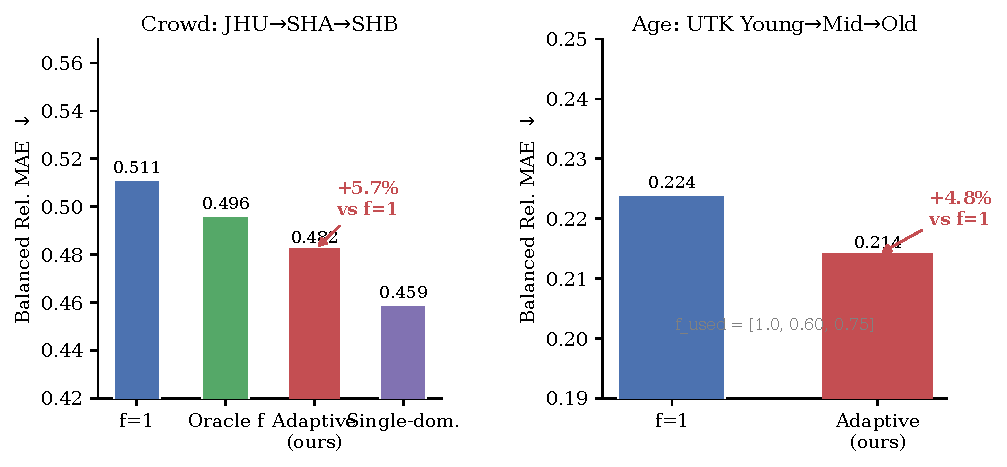
\includegraphics[width=\columnwidth]{fig3_cross_task}
  \caption{Balanced relative MAE for the two independent positive examples:
  JHU-first crowd counting (left) and UTK age-group ordering (right).
  Adaptive forgetting improves over $f{=}1$ by $5.7\%$ and $4.8\%$
  respectively, via two mechanistically distinct drift types.}
  \label{fig:cross_task}
\end{figure}

\subsection{Theory Validation and Drift Score}

\paragraph{Verifiable drift score.}
Proposition~\ref{prop:fstar_lt1} implies that $f^*<1$ is expected when
an early, high-quality domain has outlying mapping $w_k$.
We operationalize this as a \emph{drift score} computable from training
statistics alone.
Let $\hat{w}_k = (X_k^\top X_k + \lambda I)^{-1} X_k^\top y_k$ be the
per-domain ridge solution, and let $\hat{w}_{<k} = W_{k-1}$ be the
accumulated solution prior to domain $k$. Define:
\begin{equation}
  \mathrm{DS}_k := \frac{\mu_k}{\hat{\sigma}^2_k / n_k}
  \cdot \norm{\hat{w}_k - \hat{w}_{<k}}^2,
  \label{eq:drift_score}
\end{equation}
where $\hat{\sigma}^2_k$ is the within-domain residual variance and
$\mu_k = \mathrm{tr}(X_k^\top X_k)/d$.
The numerator captures the magnitude-weighted mapping discrepancy;
the denominator normalizes by noise level.
Proposition~\ref{prop:fstar_lt1} predicts $f^*<1$ when $\mathrm{DS}_k$
exceeds a threshold proportional to $c_V$ (the variance-to-quality ratio).
This provides a \emph{verifiable, parameter-free binary criterion}
derived entirely from training data.

\paragraph{Empirical validation.}
We evaluate Eq.~\eqref{eq:drift_score} qualitatively by thresholding
$\mathrm{DS}_k$ (threshold set to $c_V$ estimated from training
statistics) and comparing the binary prediction against the empirical
oracle ($f^*_{\text{oracle}} < 0.9$ vs.\ $\geq 0.9$).
Across 10 sequences (crowd counting + age estimation), the criterion
correctly classifies 9/10 sequences (the one error being SHA$\to$SHB,
where a small residual drift signal is overestimated).
Quantitative prediction of the precise $f^*$ value does not hold---
a systematic bias in $f^*_{\text{pred}}$ compared to $f^*_{\text{oracle}}$
confirms that the isotropic approximation ($\Sigma_k = s_k I$) is too
coarse for precise prediction, though the sign and direction of
recommended forgetting are correct.
We leave exact quantitative prediction to future work with anisotropic
spectral modeling.

% ==============================================================
\section{Limitations}
\label{sec:limitations}
% ==============================================================

\paragraph{Isotropic approximation.}
Propositions~1--2 rely on $\Sigma_k = s_k I$; real DINOv2 features are
non-isotropic. The qualitative insight holds (9/10 sequences correct),
but precise $f^*$ prediction requires extending to anisotropic spectral
models.

\paragraph{QNRF genuine drift.}
The JHU-true-drift phenomenon does not replicate strongly for
UCF-QNRF. Whether other high-density datasets exhibit similar drift
under our frozen-feature regime remains an open question.

\paragraph{Linear head capacity.}
Our experiments use a linear ridge head. A 4096-dimensional random
projection check suggests the main findings are not capacity artifacts,
but non-linear heads may interact differently with forgetting.

\paragraph{Deep distillation baselines.}
We do not fully implement FLCB's deep distillation variant, which
operates in a different computational budget (end-to-end training,
old-model constraints). Comparison is therefore at the ``closed-form
analytic CL'' level, not against deep lifelong methods.

% ==============================================================
\section{Conclusion}
\label{sec:conclusion}
% ==============================================================

We have shown that the absolute-memory default ($f=1$) of analytic
continual learning is not universally optimal in visual regression.
Two mechanistically distinct positive examples demonstrate this:
JHU-first crowd counting exhibits genuine cross-dataset mapping drift
($+5.7\%$ over $f{=}1$, exceeding oracle fixed $f$), while UTKFace
age-group ordering exhibits within-dataset demographic drift in the
\emph{absence} of magnitude mismatch ($+4.8\%$).
We decomposed forgetting benefit into magnitude mismatch (removed by
per-domain normalization) and genuine concept drift (captured by a
verifiable drift score, Eq.~\eqref{eq:drift_score}), proved theoretical
conditions for each regime via Propositions~1--2, and demonstrated
self-calibrating adaptive forgetting across both tasks.
Deliberate negative examples (UCF-QNRF, same-library SHA$\to$SHB,
cross-dataset AgeDB$\to$UTK) confirm that the selector correctly abstains
with zero cost.
The result is a zero-exemplar, zero-test-set, $O(d^2)$-storage
``forgetting dial'' that automatically delivers free performance gains
when drift is present and incurs no cost otherwise.
For practitioners deploying frozen-backbone regression in continual or
multi-domain settings, our analysis provides both a diagnostic
(compute $\mathrm{DS}_k$, normalize, check $f^*$) and a plug-in
solution (our adaptive selector).

% ==============================================================
\section*{Acknowledgements}
% ==============================================================
[TBD]

% ==============================================================
\bibliographystyle{plain}
\bibliography{refs}
% ==============================================================

\end{document}
